\documentclass{standalone}

\usepackage[english]{babel}
\usepackage[linesnumbered, ruled, vlined]{algorithm2e}

\usepackage{caption}

% to create listings

\usepackage{listings, lstautogobble}
\lstset{
  autogobble=true,
  frame=single,
}

\lstdefinelanguage{coq}[Objective]{Caml}{
  morekeywords={Structure, Definition, Inductive, list, return},
  sensitive=true
}

% to define font size

\usepackage{ulem}
\usepackage{moresize}
\usepackage{anyfontsize}

% to use tikz and its libraries

\usepackage{tikz-timing}
\usepackage{tikz}

\usetikzlibrary{backgrounds}
\usetikzlibrary{positioning, calc, arrows, shapes, automata, petri, patterns}

% to use tikzmark, to place and refer to marks outside the current figure

\tikzset{every picture/.style={remember picture}}

% styles for transitions

\tikzset{transition/.append style={fill=black!20, thick}}
\tikzset{transition/.append style={fill=black!20, thick}}

% styles for test and inhib arcs.

\tikzstyle{test}=[pre, *-]
\tikzstyle{inhib}=[pre, o-]

% to use colors

\usepackage{xcolor}

%%%%%%%%%%%%%%%%%%%%%%%%%%%%%%%%%%%%%%%%%%%%%%%%%%
%                  BEGIN DOCUMENT                %
%%%%%%%%%%%%%%%%%%%%%%%%%%%%%%%%%%%%%%%%%%%%%%%%%%

\begin{document}

\begin{tikzpicture}

  % \node (pn1) {
  %   \begin{tikzpicture}
  %     \node[place, tokens=1] (p0) [label={above:$p$}] {};
      
  %     \node[transition, anchor=north east] (t0) at ($(p0.south west)-(.5,.5)$) {}
  %     edge[pre, bend left] (p0);
  %     \node[anchor=east] at ($(t0.west)$) {
  %       \begin{tabular}{@{}c@{}}
  %         $t_0$ \\
  %         $[2,4]$ \\
  %       \end{tabular}
  %     };

  %     \node[transition, anchor=north west] (t2) at ($(p0.south east)+(.5,-.5)$) {}
  %     edge[pre, bend right] (p0);
  %     \node[anchor=west] at ($(t2.east)$) {
  %       \begin{tabular}{@{}c@{}}
  %         $t_1$ \\
  %         $[5,\infty]$ \\
  %       \end{tabular}
  %     };

  %   \end{tikzpicture}    
  % };

  % \node[anchor=north, draw, circle, inner sep=1pt] at (pn1.south) {1};

  \node (pn2) {
    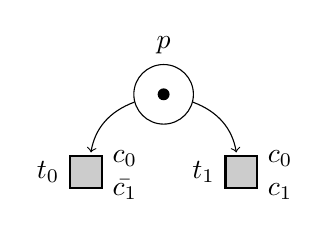
\begin{tikzpicture}
      \node[place, tokens=1] (p0) [label={above:$p$}] {};
      
      \node[transition, anchor=north east] (t0) at ($(p0.south west)-(.5,.5)$) {}
      edge[pre, bend left] (p0);
      \node[anchor=east] at ($(t0.west)$) {$t_0$};
      \node[anchor=west] at ($(t0.east)$) {
        \begin{tabular}{@{}c@{}}
          $c_0$ \\
          $\bar{c_1}$ \\
        \end{tabular}
      };

      \node[transition, anchor=north west] (t2) at ($(p0.south east)+(.5,-.5)$) {}
      edge[pre, bend right] (p0);
      \node[anchor=east] at ($(t2.west)$) {$t_1$};
      \node[anchor=west] at ($(t2.east)$) {
        \begin{tabular}{@{}c@{}}
          $c_0$ \\
          $c_1$ \\
        \end{tabular}
      };
      
    \end{tikzpicture}    
  };

  \node[anchor=north, draw, circle, inner sep=1pt] at (pn2.south) {1};

  \node (pn3) at ($(pn2.east)+(1.5,0)$) {
    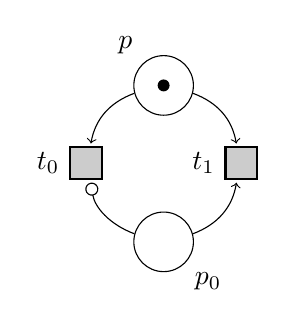
\begin{tikzpicture}
      \node[place, tokens=1] (p0) [label={above left:$p$}] {};
      
      \node[transition, anchor=north east] (t0) at ($(p0.south west)-(.5,.5)$) {}
      edge[pre, bend left] (p0);
      \node[anchor=east] at ($(t0.west)$) {$t_0$};

      \node[transition, anchor=north west] (t2) at ($(p0.south east)+(.5,-.5)$) {}
      edge[pre, bend right] (p0);
      \node[anchor=east] at ($(t2.west)$) {$t_1$};

      \node[place] (p1) at ($(t0)!.5!(t2)-(0,1)$) [label={below right: $p_0$}] {};
      
      \draw (t0) edge[inhib, bend right] (p1);
      \draw (t2) edge[pre, bend left] (p1);
      
    \end{tikzpicture}    
  };

  \node[anchor=north, draw, circle, inner sep=1pt] at (pn3.south) {2};
  
\end{tikzpicture}

\end{document}
%%% Local Variables:
%%% mode: latex
%%% TeX-master: t
%%% End:
